\chapter{METODOLOGIA E ATIVIDADES REALIZADAS}
\label{cap:atividades}

\section{Caracterização metodológica}
\label{sec:metodo}

Trata-se de uma ação de natureza aplicada, com abordagem qualitativa e quantitativa e caráter exploratório. O desenvolvimento seguiu uma prototipagem incremental: cada funcionalidade foi implementada, gravada na placa, testada e ajustada antes da etapa seguinte. Os testes combinaram observação direta do comportamento do protótipo (se a interface detectava, anunciava e atualizava os pontos) com registros numéricos obtidos pela saída serial do ESP32. Todo o código foi versionado em repositório Git, o que permite reconstituir a sequência das atividades descritas a seguir.

\section{Materiais utilizados}
\label{sec:materiais}

O Quadro~\ref{qua:materiais} lista os materiais e as ferramentas usados até esta etapa.

\begin{quadro}[htb]
\caption{Materiais e ferramentas utilizados}
\label{qua:materiais}
\small
\begin{tabular}{|p{5.8cm}|p{8.2cm}|}
\hline
\textbf{Item} & \textbf{Uso no projeto} \\
\hline
2 placas ESP32-C3 SuperMini (4~MB de flash) & Uma como bracelete e outra como baliza fixa \\
\hline
\textit{Smartphone} Android com navegador Chrome & Execução da interface web (Web Bluetooth e voz) \\
\hline
Notebook com Linux e adaptador Bluetooth & Compilação, gravação, coleta de registros e simulação de balizas \\
\hline
arduino-cli 1.5.2 e núcleo Arduino-ESP32 3.3.11 & Compilação e gravação do firmware pela linha de comando \\
\hline
Aplicativo nRF Connect (Nordic Semiconductor) & Inspeção dos serviços BLE e validação das notificações \\
\hline
BlueZ (\texttt{bluetoothctl}) & Uso do notebook como baliza BLE nos testes \\
\hline
Python 3 com biblioteca pyserial & Leitura e resumo dos registros da porta serial \\
\hline
Git, GitHub e GitHub Pages & Versionamento do código e hospedagem da interface em HTTPS \\
\hline
Bateria LiPo 3,7~V & Prevista no projeto físico; montagem pendente \\
\hline
Motor de vibração tipo moeda & Uso em avaliação; saída PWM já prevista no firmware \\
\hline
\end{tabular}
\normalsize
\fonte{Elaborado pelos autores (2026).}
\end{quadro}

\section{Arquitetura do sistema}
\label{sec:arquitetura}

A Figura~\ref{fig:arquitetura} mostra a arquitetura adotada. As balizas apenas anunciam seu nome. O bracelete recebe esses anúncios, calcula a distância de cada baliza e repassa a lista ao celular. O celular apenas recebe os dados e os apresenta ao usuário, por voz, vibração do aparelho e texto em alto contraste. O firmware já possui uma saída PWM para um motor de vibração no bracelete, cujo uso ainda está em avaliação.

\begin{figure}[htb]
\centering
\caption{Arquitetura do sistema e sentido do fluxo de dados}
\label{fig:arquitetura}
\begin{tikzpicture}[
    bloco/.style={draw, rounded corners, thick, align=center, minimum width=3.6cm, minimum height=2.1cm, font=\small},
    seta/.style={-{Stealth[length=3mm]}, thick},
    rot/.style={font=\footnotesize, align=center}
]
\node[bloco] (baliza) {\textbf{Balizas BLE}\\ESP32-C3 ou \textit{beacon}\\nome \texttt{BALIZA-<Nome>}\\anúncio a cada 100~ms};
\node[bloco, right=2.3cm of baliza] (bracelete) {\textbf{Bracelete}\\ESP32-C3\\varredura + RSSI\\estimativa de distância};
\node[bloco, right=2.3cm of bracelete] (celular) {\textbf{\textit{Smartphone}}\\página web\\lista em alto contraste\\voz e vibração};
\draw[seta] (baliza) -- node[rot, above] {anúncios\\BLE} (bracelete);
\draw[seta] (bracelete) -- node[rot, above] {notificação\\GATT} (celular);
\node[rot, below=0.25cm of bracelete] {sem escrita: o celular não envia comandos};
\end{tikzpicture}
\fonte{Elaborado pelos autores (2026).}
\end{figure}

\section{Etapa 1 -- Concepção física e mudança de escopo}
\label{sec:etapa1}

A primeira versão do projeto seguia a proposta: um sensor ultrassônico HC-SR04 mediria a distância até obstáculos e o motor vibraria com intensidade proporcional. Um primeiro firmware com essa lógica chegou a ser escrito para o ESP32. No detalhamento do projeto, porém, a equipe decidiu retirar o sensor, com dois objetivos: simplificar o hardware do bracelete e concentrar a solução na comunicação sem fio que o ESP32 já oferece. A Figura~\ref{fig:esquema} mostra a concepção física elaborada nessa fase, com microcontrolador, bateria LiPo de 3,7~V, botão liga/desliga e um motor de vibração tipo moeda. O uso desse motor ainda está em avaliação pela equipe, e nesta etapa o retorno ao usuário é dado pelo celular.

\begin{figure}[htb]
\centering
\caption{Esquema técnico da concepção física do bracelete}
\label{fig:esquema}
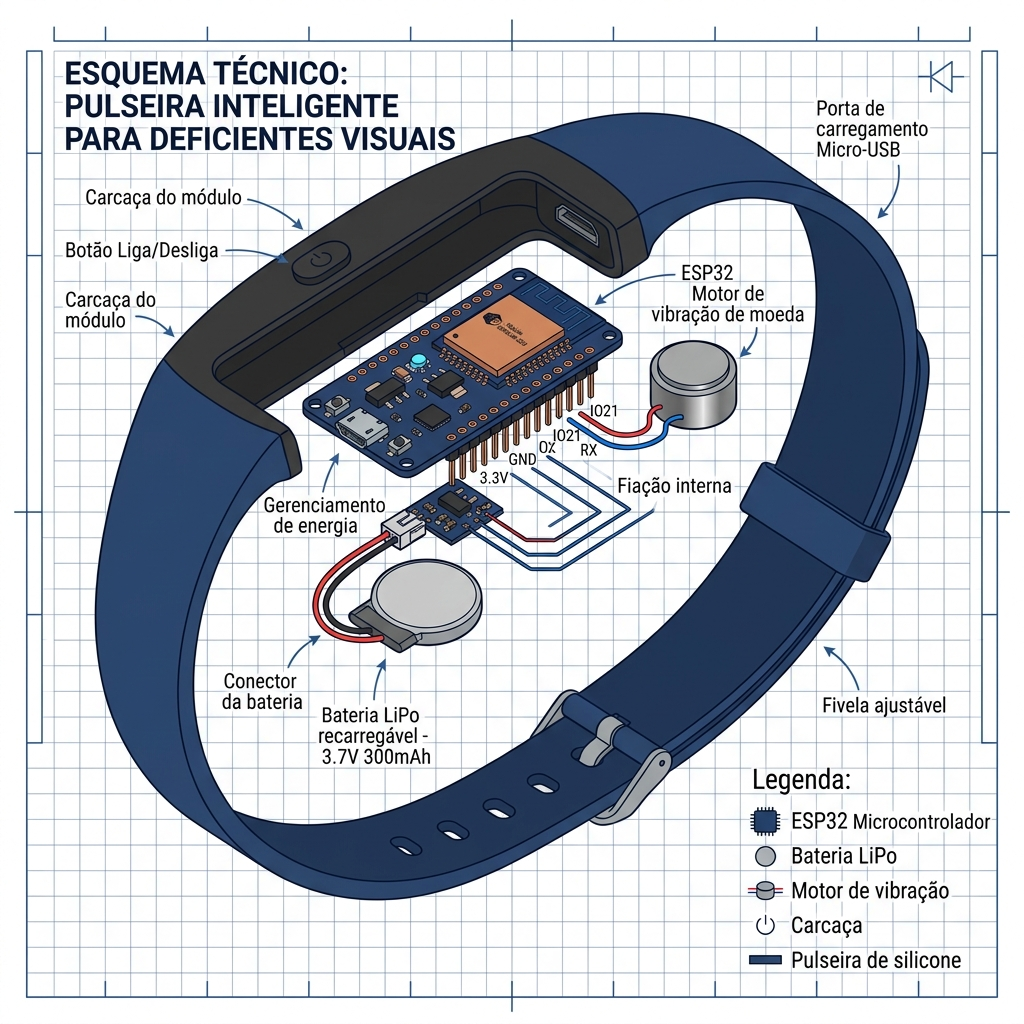
\includegraphics[width=0.62\textwidth]{figuras/esquema_tecnico.jpg}
\fonte{Elaborado pelos autores (2026).}
\end{figure}

Com essa configuração, era preciso outra forma de perceber o ambiente. A alternativa escolhida foi aproveitar o rádio Bluetooth que o ESP32 já possui: pontos de referência do ambiente recebem balizas BLE, e o bracelete estima a proximidade de cada uma pelo sinal. A abordagem não exige componentes extras no bracelete. Em contrapartida, só funciona em ambientes onde as balizas foram instaladas.

\section{Etapa 2 -- Comunicação BLE do bracelete para o celular}
\label{sec:etapa2}

Um requisito definido pela equipe foi que a comunicação ocorresse apenas no sentido bracelete $\rightarrow$ celular. Para isso, o ESP32 foi configurado como servidor GATT com um serviço próprio, identificado por UUID, contendo uma única característica com as propriedades de leitura e notificação e sem escrita. Quando o celular se inscreve nas notificações, o bracelete passa a enviar os dados a cada 500~ms. A comunicação foi validada primeiro com o aplicativo nRF Connect, que exibiu o dispositivo \texttt{Bracelete-ESP32} e os valores recebidos por notificação.

\section{Etapa 3 -- Interface web no celular}
\label{sec:etapa3}

Para dispensar a instalação de aplicativo, a interface foi feita como uma página web estática que usa Web Bluetooth para se conectar ao bracelete. A página foi publicada no GitHub Pages, que fornece o HTTPS exigido pela API. O desenho da interface seguiu três princípios voltados à baixa visão:
\begin{itemize}
    \item fundo preto com texto grande e cores de alto contraste;
    \item cores diferentes por faixa de proximidade;
    \item anúncio por voz das mudanças.
\end{itemize}
Um botão ``O que tem por perto?'' lê em sequência todos os pontos detectados, do mais próximo para o mais distante. A Figura~\ref{fig:interface} mostra a versão atual da interface.

\begin{figure}[htb]
\centering
\caption{Interface web exibindo três pontos no modo demonstração}
\label{fig:interface}
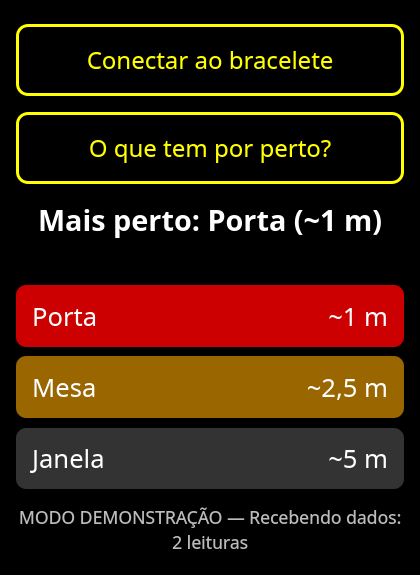
\includegraphics[width=0.36\textwidth]{figuras/interface_web_demo.png}
\fonte{Elaborado pelos autores (2026). Captura em navegador de computador, com mensagem no formato enviado pelo bracelete no modo demonstração.}
\end{figure}

Uma decisão de segurança foi tomada durante os testes. A primeira versão exibia ``Caminho livre'' quando o sensor não retornava leitura, o que poderia induzir o usuário a erro. A interface passou a diferenciar a ausência de leitura, informando ``Nenhuma baliza por perto'', e nunca anuncia caminho livre.

\section{Etapa 4 -- Migração para o ESP32-C3}
\label{sec:etapa4}

O firmware foi escrito inicialmente para o ESP32 convencional. A placa disponível, porém, era um ESP32-C3, identificado pela ferramenta \texttt{esptool}, o que exigiu três ajustes:
\begin{itemize}
    \item \textbf{pinos:} os GPIO 18 e 19, usados antes, correspondem ao USB nativo do C3, e os GPIO 2, 8 e 9 são pinos de inicialização. A saída reservada ao motor foi movida para o GPIO~5;
    \item \textbf{saída serial:} foi necessário habilitar a opção \textit{USB CDC On Boot} para que a saída serial fosse enviada pela USB;
    \item \textbf{PWM:} as funções de PWM foram atualizadas para a API da versão 3 do núcleo Arduino-ESP32.
\end{itemize}
Para simplificar a gravação sem a IDE do Arduino, foi criado um \textit{script} que compila, grava e abre o monitor serial com o \texttt{arduino-cli}.

\section{Etapa 5 -- Modo demonstração}
\label{sec:etapa5}

Para permitir apresentações sem depender de balizas instaladas, foi criado um modo demonstração, ligado e desligado pelo botão BOOT da placa. Nesse modo, o bracelete simula três balizas (``Porta'', ``Mesa'' e ``Janela'') com distâncias que variam ciclicamente, e a interface indica claramente ``MODO DEMONSTRAÇÃO'' para não ser confundida com uma leitura real. O modo sempre inicia desligado.

\section{Etapa 6 -- Detecção de múltiplas balizas}
\label{sec:etapa6}

Nesta etapa foi implementada a detecção por balizas, com dois programas:
\begin{itemize}
    \item \textbf{Firmware da baliza:} o ESP32-C3 anuncia o nome \texttt{BALIZA-<Nome>} a cada 100~ms, com potência de transmissão fixa, para que a relação entre sinal e distância seja estável;
    \item \textbf{Firmware do bracelete:} faz varredura contínua ativa, com janela de 50~ms a cada 100~ms, deixando tempo de rádio para a conexão com o celular. Ele mantém uma tabela de até oito balizas com o RSSI suavizado pela Equação~\ref{eq:ema}, usando $\alpha = 0{,}15$, e descarta a baliza que fica mais de 6~s sem ser ouvida.
\end{itemize}

A distância é calculada pela Equação~\ref{eq:distancia}, com valores iniciais $A = -59$~dBm e $n = 2{,}5$, e classificada em três faixas (até 1~m, até 2~m e até 4~m). Para evitar que os alertas fiquem alternando na fronteira de uma faixa, foi aplicada uma histerese: para voltar a uma faixa mais distante, a estimativa precisa ultrapassar o limite em 25\%.

A mensagem enviada ao celular segue o formato \texttt{<demo>|Nome:cm;Nome:cm;...}, com as balizas ordenadas da mais próxima para a mais distante e limitada ao tamanho máximo do pacote negociado na conexão (MTU). Na interface, um ponto novo só é anunciado após duas leituras seguidas. O mesmo ponto não é anunciado de novo em menos de 4~s, e as falas entram em fila em vez de interromper a anterior. Apenas a aproximação a menos de 1~m interrompe a fala em andamento, por ser o alerta mais urgente. O Apêndice~\ref{ap:codigo} traz os principais trechos do código.

\section{Etapa 7 -- Procedimentos de teste}
\label{sec:etapa7}

Os testes foram feitos de forma incremental, após cada etapa:
\begin{enumerate}
    \item \textbf{compilação:} todos os programas foram compilados e o uso de memória foi registrado;
    \item \textbf{comunicação:} o bracelete foi conectado ao nRF Connect e depois à interface web, verificando a chegada das notificações;
    \item \textbf{balizas simuladas:} o notebook foi configurado com o BlueZ para anunciar uma e depois duas balizas, e a saída serial do bracelete foi registrada por cerca de 45~s com um \textit{script} em Python, que contou as leituras e as entradas e saídas de balizas;
    \item \textbf{baliza real:} a segunda placa ESP32-C3 foi gravada como baliza ``Porta'' e posicionada a diferentes distâncias do bracelete, observando a distância indicada na interface.
\end{enumerate}
